\pdfminorversion=7
\documentclass{beamer}%[10]
\usepackage{pgf}
\usepackage[english]{babel}
\usepackage[utf8]{inputenc}
\usepackage{beamerthemesplit}
\usepackage{graphics,epsfig, subfigure}
\usepackage{url}
\usepackage{srcltx}
\usepackage{hyperref}
\usepackage{tikz,times}
%\usepackage{media9}
\usepackage{multimedia}
%\usepackage{flashmovie}
\usetikzlibrary{mindmap,backgrounds}


\definecolor{kugreen}{RGB}{0,180,114}%{50,93,61} 
\definecolor{kugreenlys}{RGB}{132,158,139}
\definecolor{kugreenlyslys}{RGB}{173,190,177}
\definecolor{kugreenlyslyslys}{RGB}{0,135,114}%{214,223,216}
\setbeamercovered{transparent}
\mode<presentation>
\usetheme[numbers,totalnumber,compress,sidebarshades]{PaloAlto}
\setbeamertemplate{footline}[frame number]
 
  \usecolortheme[named=kugreen]{structure}
  \useinnertheme{circles}
  \usefonttheme[onlymath]{serif}
  \setbeamercovered{transparent}
  \setbeamertemplate{blocks}[rounded][shadow=true]
\logo{
\includegraphics[width=1.5cm]{figs/logo_branca2}}
\setbeamercolor{logo}{bg=kugreenlyslyslys}
%\useoutertheme{infolines} 

\title{The Embedded Electronics and Software of the DORIS Offshore Robot}
\author[Renan S. Freitas]{\parbox[t]{4cm}{Renan S. Freitas\\ Marco F.S.
Xaud\\ Ighor Marcovistz\\ Alex F.
Neves\\ Rafael O. Faria\\ Guilherme Carvalho\\ Liu Hsu\\
Eduardo Nunes}\parbox[t]{4cm}{ Alessandro Peixoto \\ Fernando
Lizarralde\\
Gustavo M Freitas\\ Ramon R. Costa\\ Pål Johan From\\ Mauricio Galassi\\ Peter W. J.
Derks\\ Anders Røyrøy}}
\institute{UFRJ, PETROBRAS and STATOIL}
\date{05/29/2015} 
 
 

\begin{document}
\frame{\titlepage \vspace{-0.5cm} 

}

\frame
{
\frametitle{Overview}
\tableofcontents%[pausesection]
}

\section{Team}

\frame
{
\frametitle{Team}
\begin{itemize}
  \item Laboratório de Controle e Automação, Engenharia de Aplicação e
Desenvolvimento (LEAD);
  \item Sinais, Multimídia e Telecomunicações (SMT);
  \item Financial support: Petrobras, ANP and Statoil.
\end{itemize}

\includegraphics[width=0.33\columnwidth]{figs/petrobras_logo.png}\hspace*{1cm}

\includegraphics[width=0.3\columnwidth]{figs/ANP_logo.png}\hspace*{1cm}

\includegraphics[width=0.2\columnwidth]{figs/statoil_logo.png} 
}
 
\section{Motivation and Problem}
%\frame
%{
%\frametitle{Motivation and Problem}
%\vspace*{0.5cm}
%\begin{center}
%Why Oil and Gas industry ?
%\end{center}
%\begin{center}
%\includegraphics[width=0.4\columnwidth]<2->{figs/brazilproduction.png}\hspace*{1cm}
% \includegraphics[width=0.4\columnwidth]<2->{figs/brazilconsumption.png}
%\end{center}
%} 

\frame
{
\frametitle{Motivation and Problem}
\vspace*{0.5cm}
\begin{center}
Why offshore robotics ?
\end{center}
\begin{itemize}[<+->]
  \item Atmospheric conditions;
  \item Corrosive agents;
  \item Weather;
  \item Constrained space;
  \item Profit/cost.
\end{itemize}
}

\frame
{
\frametitle{Motivation and Problem}
\begin{center}
Previous research project for offshore applications:
\end{center}
\begin{itemize}[<+->]
  \item <1-> MIMROex (Fraunhofer) ;
  \item <2> Sensabot (Carnegie Mellon University). 
\end{itemize}
\includegraphics[width=0.4\columnwidth]<1->{figs/mimroex.png}\hspace*{1cm}
\includegraphics[width=0.4\columnwidth]<2>{figs/sensabot.jpg}
}

\section{DORIS Robot}
\frame{
\frametitle{DORIS overview}
\begin{center}
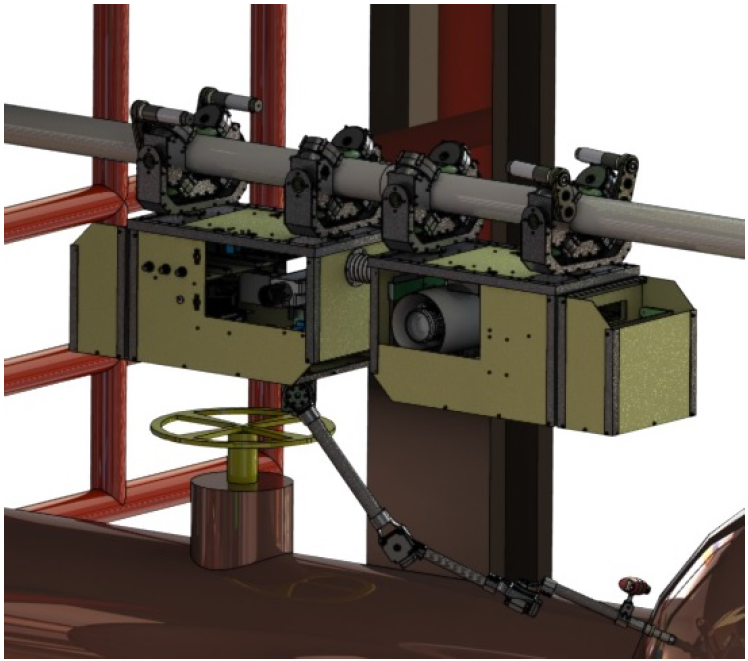
\includegraphics[width=0.8\columnwidth]{figs/DORISoverview.png}
\end{center}
} 

\subsection{DORIS overview}
\frame
{
\frametitle{DORIS overview}
\centering
\includegraphics[width=0.3\columnwidth]<1->{figs/DORISoverview.png}
\begin{itemize}[<+->]
  \item <1-> Offshore inspection and monitoring robot;
  \item <2-> Multiple sensors: a fixed, an infrared, a fisheye and a 3D cameras,
  hydrocarbon, vibration, IMU;
  \item <3-> \textit{in loco} data processing;
  \item <4-> Signal processing: intruders in restricted areas, abandoned
  objects, smoke and fire detection, liquid and gas leakage detection;
  \item <5-> Autonomous and teleoperated robot.
\end{itemize}
}

\frame
{
\frametitle{DORIS overview}
\begin{figure}
        \centering
        \resizebox {\textheight} {!} {

		\begin{tikzpicture}[mindmap,
  level 1 concept/.append style={level distance=130,sibling angle=72},
  extra concept/.append style={color=blue!50,text=black}]

  \begin{scope}[mindmap, concept color=blue, text=white]
    \node [concept] {\huge \textbf{Fields}}[clockwise from=1] 
      child {node [concept] (sof) {\textbf{Software}}}
      child {node [concept] (ele) {\textbf{Electronics}}}
      child {node [concept] (pos) {\textbf{Power supply}}}
      child {node [concept] (mec) {\textbf{Mechanics}}}
      child {node [concept] (sig) {\textbf{Signal processing}}};
      \end{scope}
\end{tikzpicture}
}
\end{figure}
}

\frame
{
\frametitle{DORIS overview}
\begin{figure}
        \centering
        \resizebox {\textheight} {!} {

		\begin{tikzpicture}[mindmap,
  level 1 concept/.append style={level distance=130,sibling angle=72},
  extra concept/.append style={color=blue!50,text=black}]

  \begin{scope}[mindmap, concept color=blue, text=white]
    \node [concept] {\huge \textbf{Fields}}[clockwise from=1] 
      child {node [concept,opacity=0.5] (sof) {\textbf{Software}}}
      child {node [concept,opacity=0.5] (ele) {\textbf{Electronics}}}
      child {node [concept,opacity=0.5] (pos) {\textbf{Power supply}}};
  \end{scope}
\end{tikzpicture}
}
\end{figure}
}
\subsection{Electronics}

\frame{
\frametitle{Electronics features}
\begin{itemize}[<+->]
\item <1-> Modularity;
\item <2-> Flexibility and reconfigurability;
\item <3-> Robustness and safety: communication and devices;
\item <4-> Device and module monitoring;
\item <5-> Autonomy and teleoperation capabilities.
\end{itemize}
}
 
\frame{
\frametitle{Actuation}
\begin{figure}
\centering
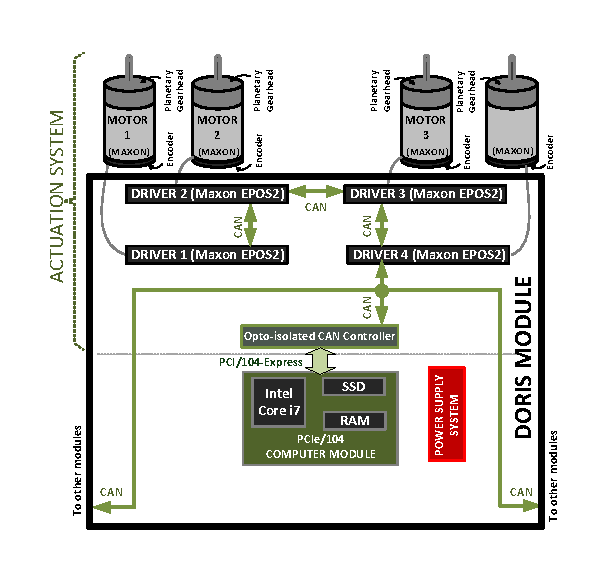
\includegraphics[width=0.8\columnwidth]{figs/DORISactsys.pdf}
\end{figure}
}

\frame{
\frametitle{Communication}
\begin{figure}
\centering
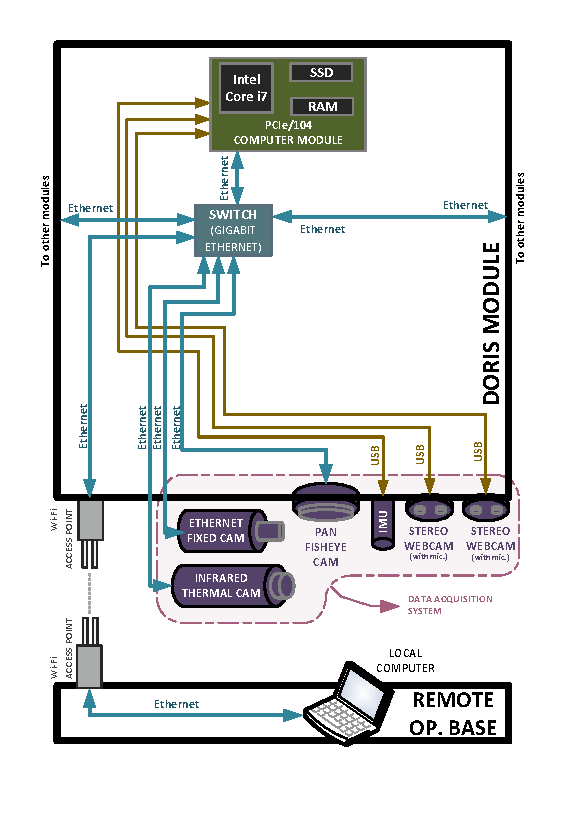
\includegraphics[width=0.5\columnwidth]{figs/DORIScommsys.pdf}
\end{figure}
}

\frame{
\frametitle{Vehicle support system}
\begin{figure}
\centering
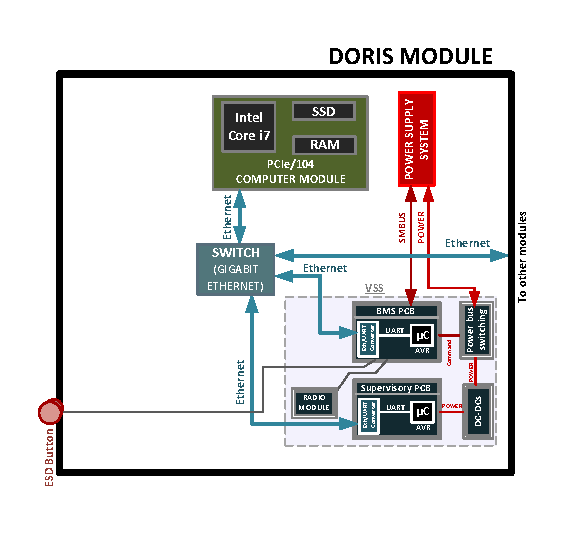
\includegraphics[width=0.8\columnwidth]{figs/DORISPCB.pdf}
\end{figure}
}

\subsection{Power Supply}

\frame{
\frametitle{Power supply features}
\begin{itemize}[<+->]
\item  Safety;
\item  Reliability;
\end{itemize}
}

\frame{
\frametitle{Power Supply}
\includegraphics[width=0.7\columnwidth]<1>{figs/DORISps1.pdf}
\includegraphics[width=0.7\columnwidth]<2>{figs/DORISps2.pdf}
\includegraphics[width=0.7\columnwidth]<3>{figs/DORISps3.pdf}
\includegraphics[width=0.7\columnwidth]<4>{figs/DORISps4.pdf}
\includegraphics[width=0.7\columnwidth]<5>{figs/DORISps5.pdf}
\includegraphics[width=0.7\columnwidth]<6>{figs/DORISps6.pdf} 
}

\subsection{Software architecture}
\frame{
\frametitle{Software features}
\begin{itemize}[<+->]
\item <1->Linux/Ubuntu is the operating system;
\item <2->Qt is the graphical interface framework;
\item <3->Robot Operating System (ROS) is the communication middleware;
\item <4->Autonomous control;
\item <5-> Remote control through GUI in the Host
Control Base (HCB) computer. HCB and robot communication by ROS nodes.
\end{itemize}
}

\frame{
\frametitle{Robot Package Software}
\begin{itemize}[<+->]
\item <1->Tools - graphical windows;
\item <2->Components - processing and communication units;
\end{itemize}
}

\frame{
\frametitle{General Package}
\includegraphics[width=1\columnwidth]<1>{figs/GP1.pdf}
\includegraphics[width=1\columnwidth]<2>{figs/GP2.pdf}
\includegraphics[width=1\columnwidth]<3>{figs/GP3.pdf}
\includegraphics[width=1\columnwidth]<4>{figs/GP4.pdf}
}

\frame{
\frametitle{DORIS Package}
\includegraphics[width=1\columnwidth]<1>{figs/DP1.pdf}
\includegraphics[width=1\columnwidth]<2>{figs/DP2.pdf}
\includegraphics[width=1\columnwidth]<3>{figs/DP3.pdf}
\includegraphics[width=1\columnwidth]<4>{figs/DORISMsoft.pdf}

}

\section{Experimental tests and resuts}
\frame{
\frametitle{Single Autonomous Module (SAM)}
%\begin{center}
%\includemedia[
%    activate=pageopen,
%    width=0.5\columnwidth]{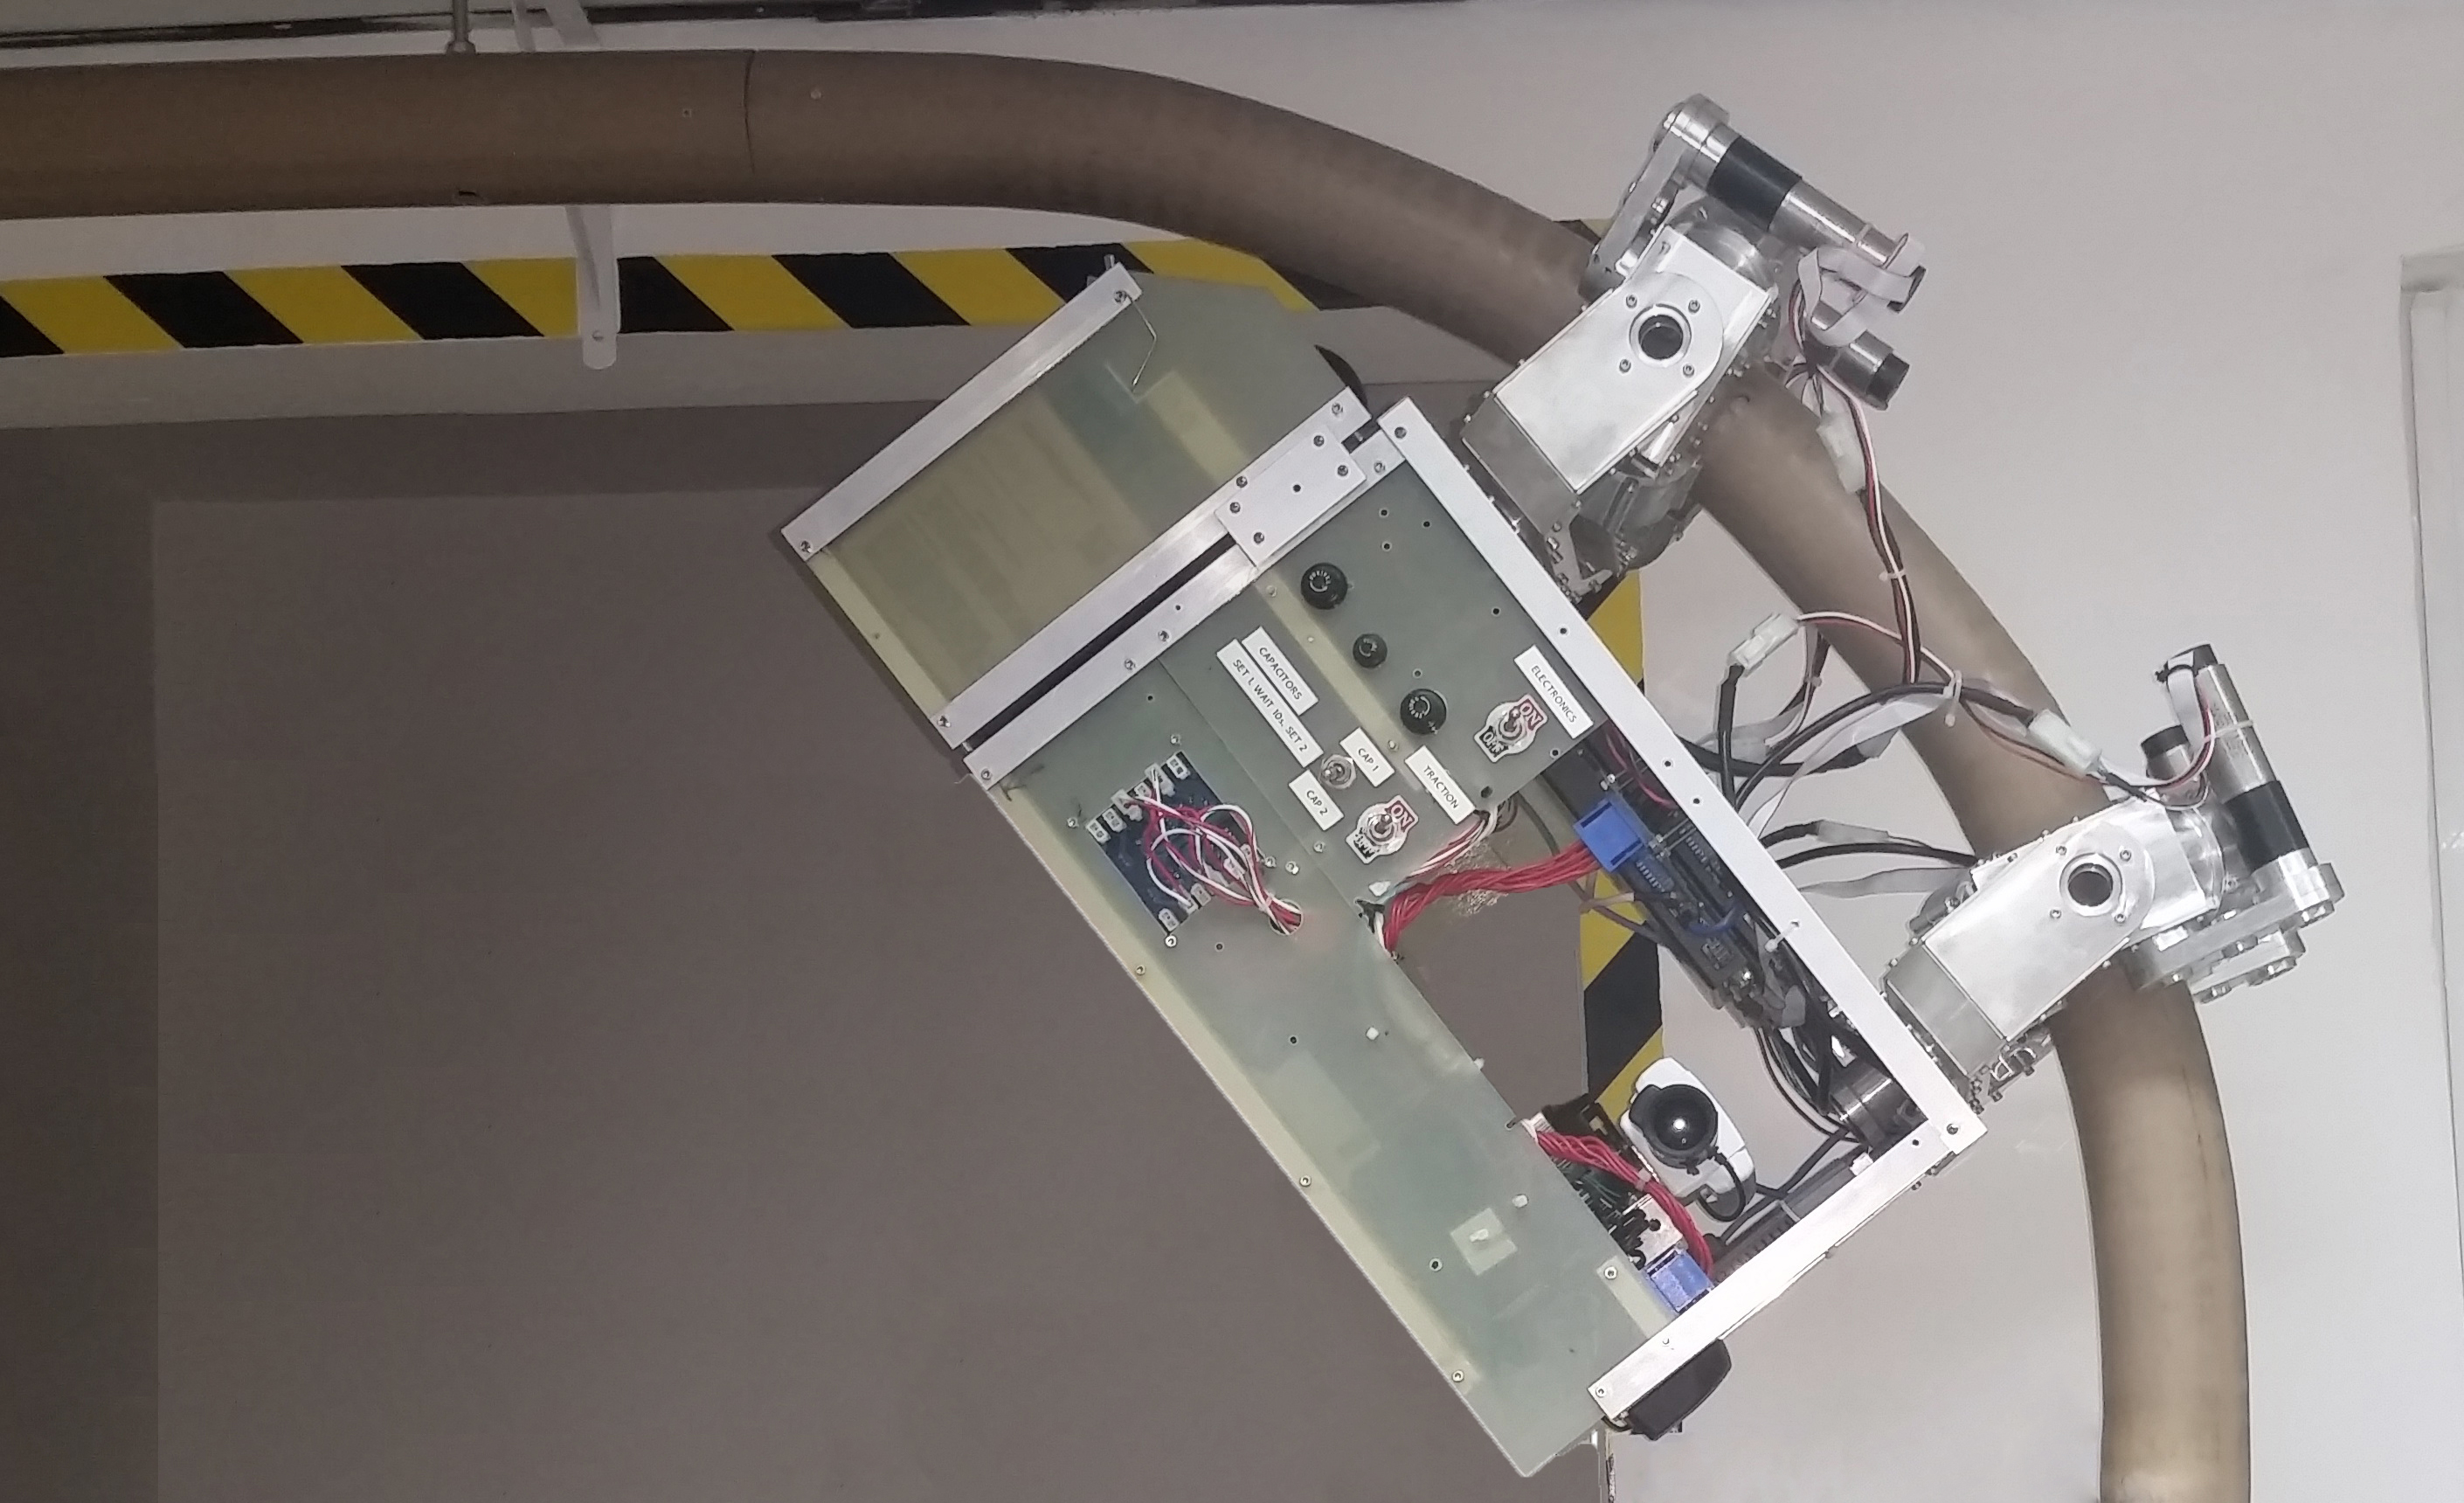
\includegraphics{figs/SAM.jpg}}{figs/dorislap.swf}
%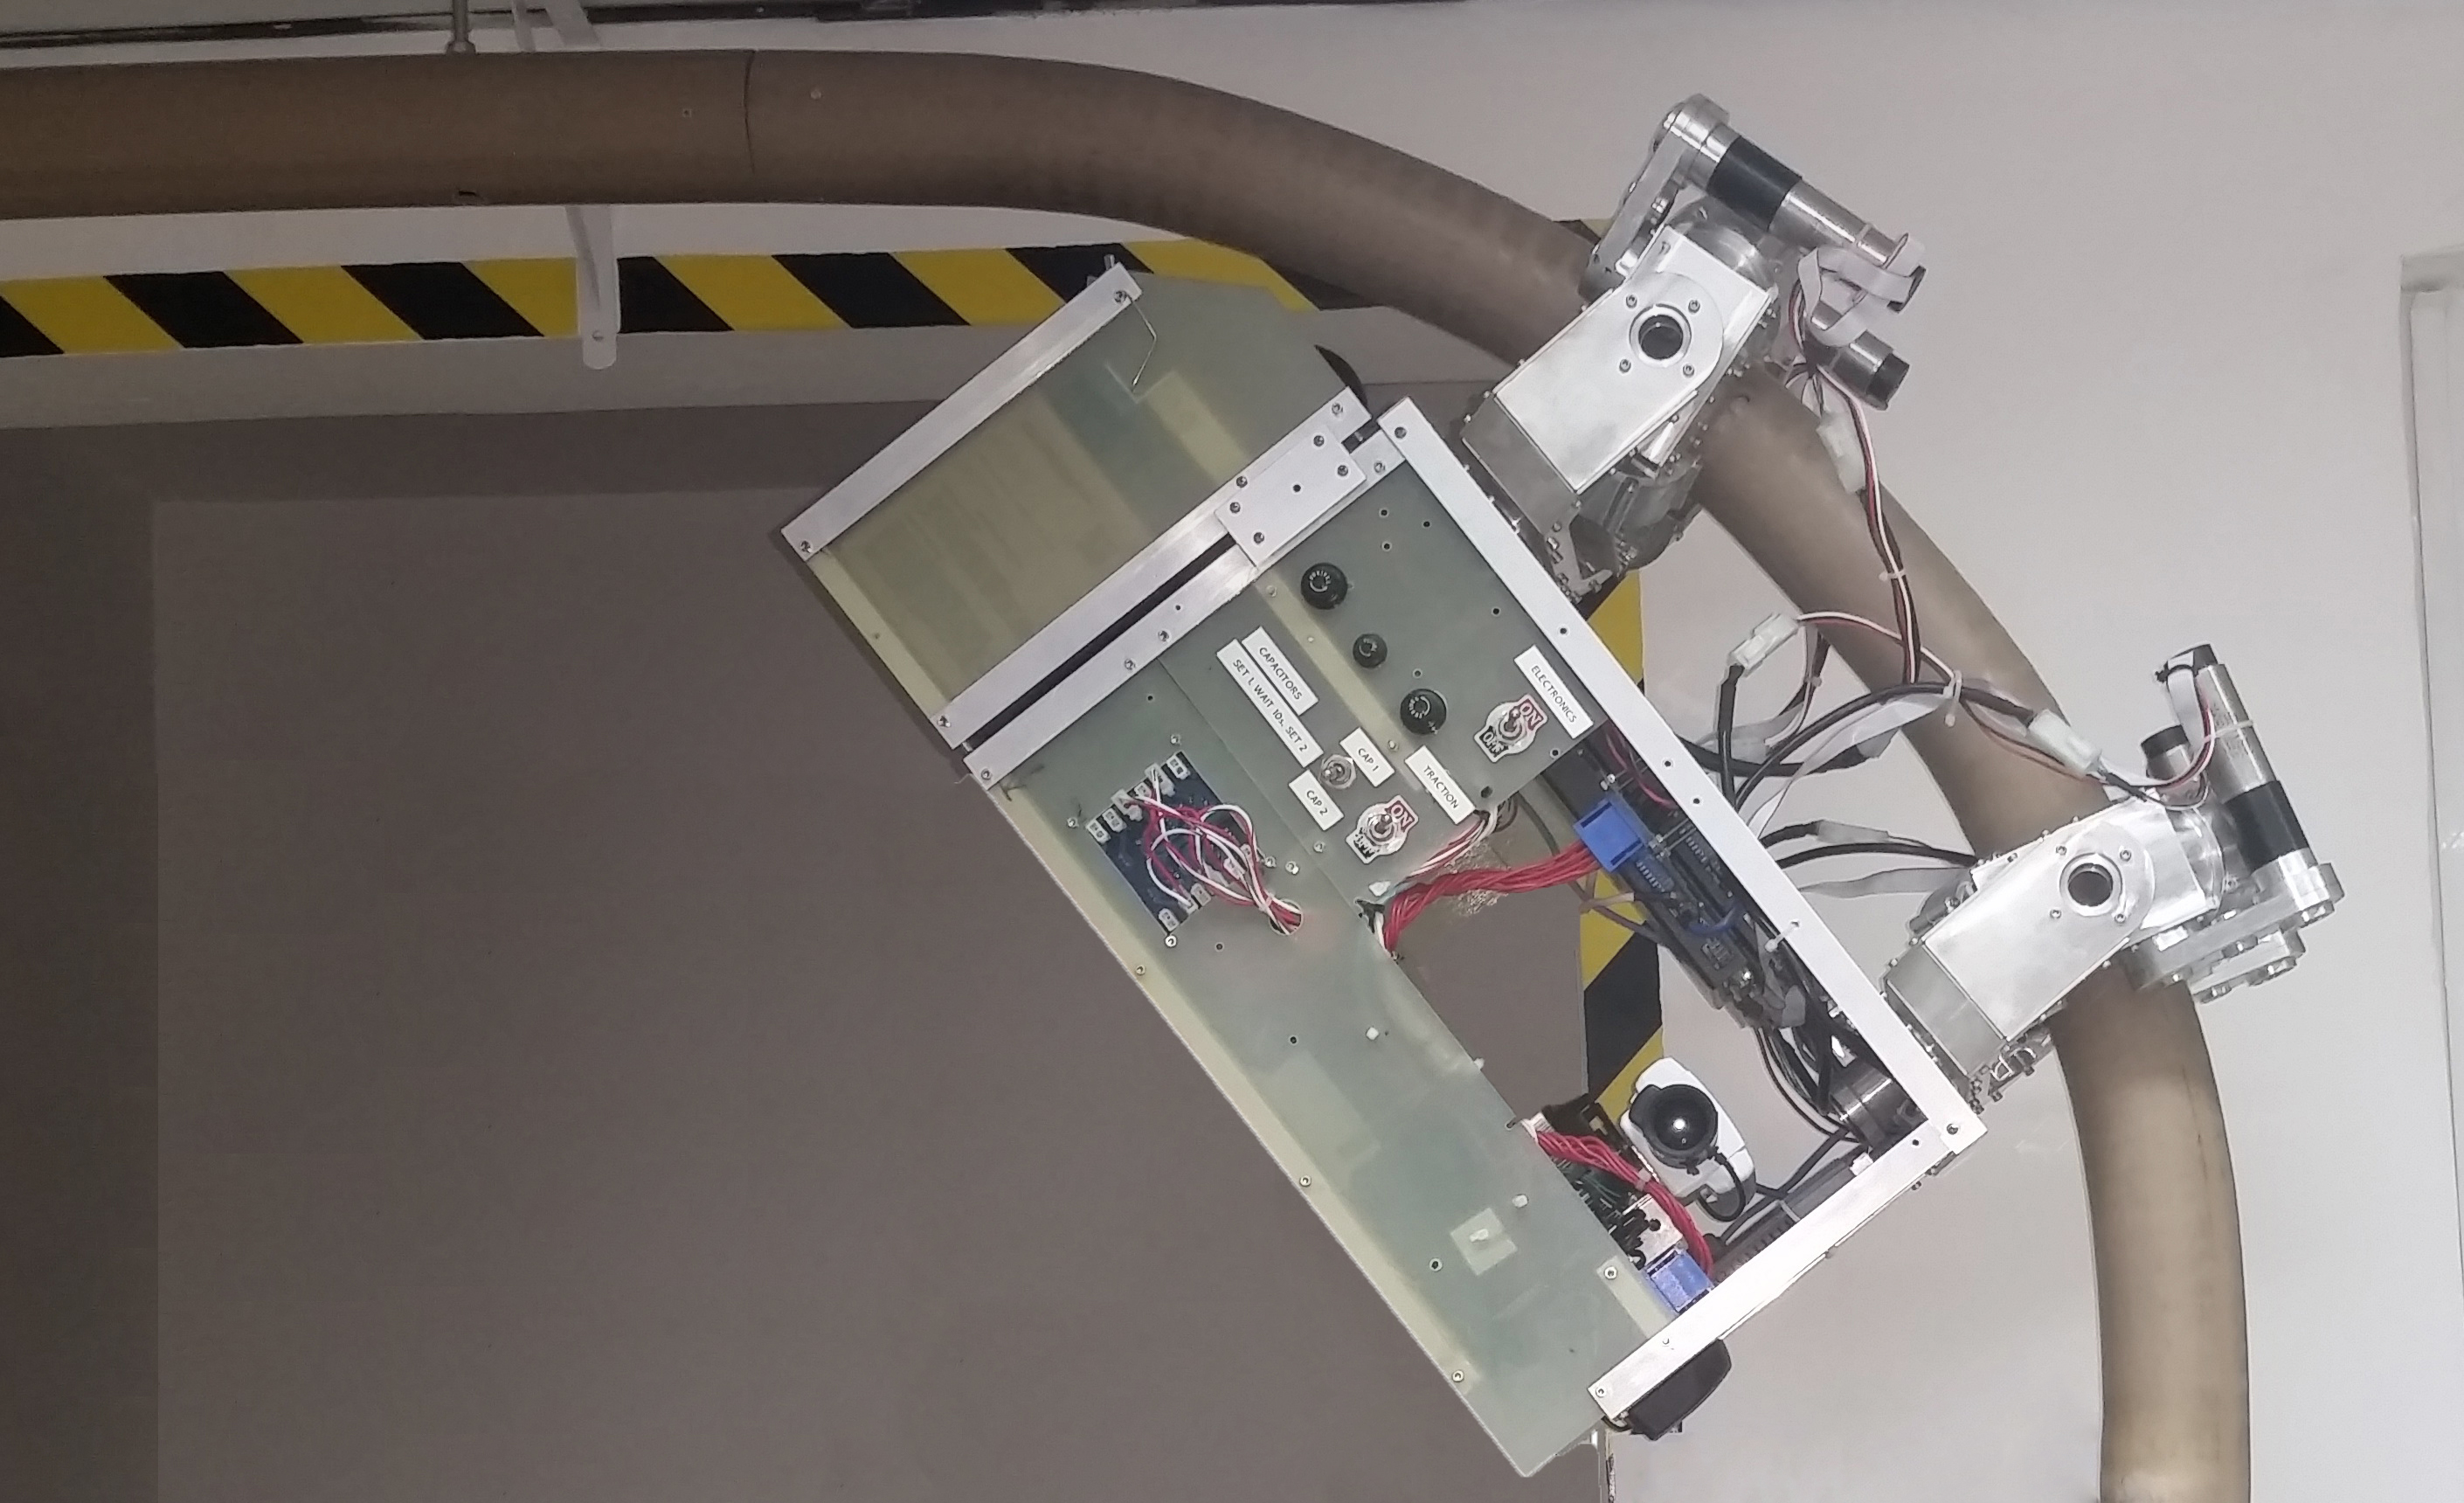
\includegraphics[width=0.5\columnwidth]{figs/SAM.jpg}
%\end{center}
\begin{center}
%\flashmovie[width=0.5\columnwidth]{figs/DORISlap.mp4}
\movie[showcontrols]{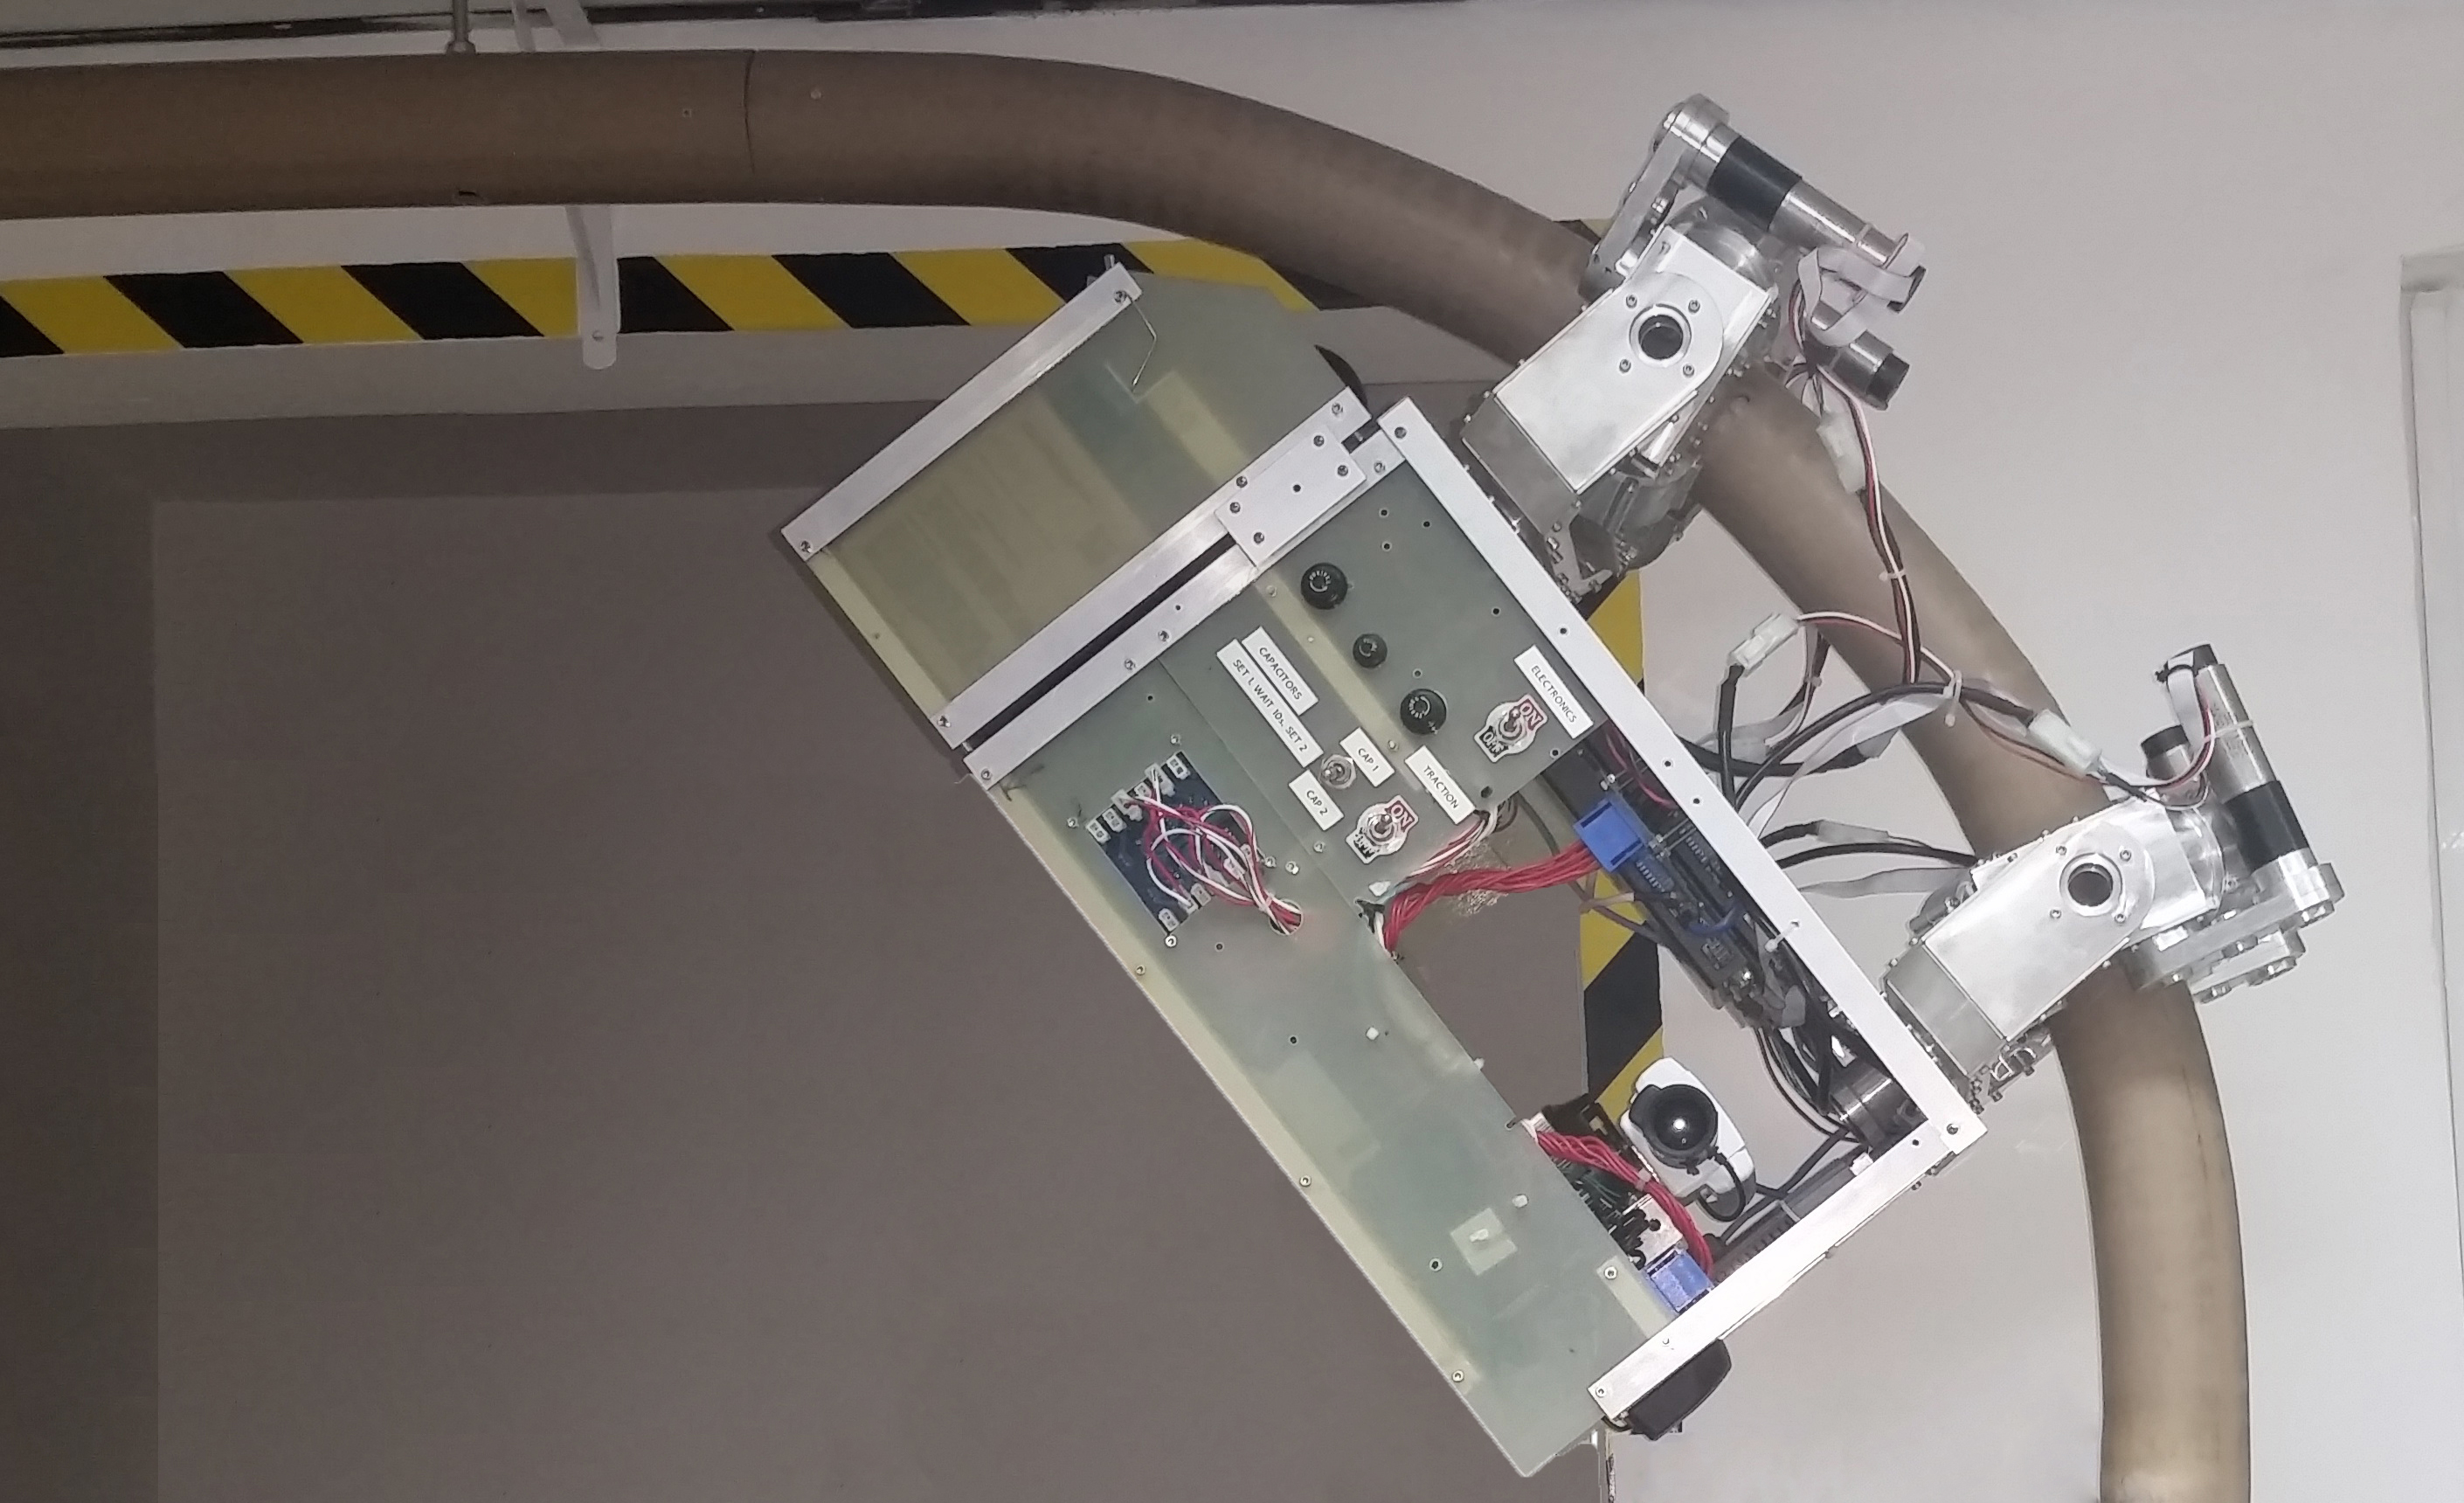
\includegraphics[width=0.5\columnwidth]{figs/SAM.jpg}}{figs/DORISlap.mp4} 
\end{center} 
\textbf{Electronics:}
\begin{itemize}[<+->]
\item <1->Actuator system: 4 brushless motors, Maxon drivers, CAN interface; 
\item <2->Data acquisition: PC104, Fixed and 3D cameras, IMU, WiFi router
(Ethernet);
\item <3->Sensor integration and communication;
\item <4->VSS implemented and tested.
\end{itemize}
}
%\frame{
%\frametitle{VSS implementation and tests}
%\includegraphics[width=\columnwidth]<1>{figs/SMBUS2.png}
%\includegraphics[width=\columnwidth]<2>{figs/SMBUS3.png}
%\includegraphics[width=\columnwidth]<3>{figs/relay.png}
%}

\frame{
\frametitle{Single Autonomous Module (SAM)}
\begin{center}
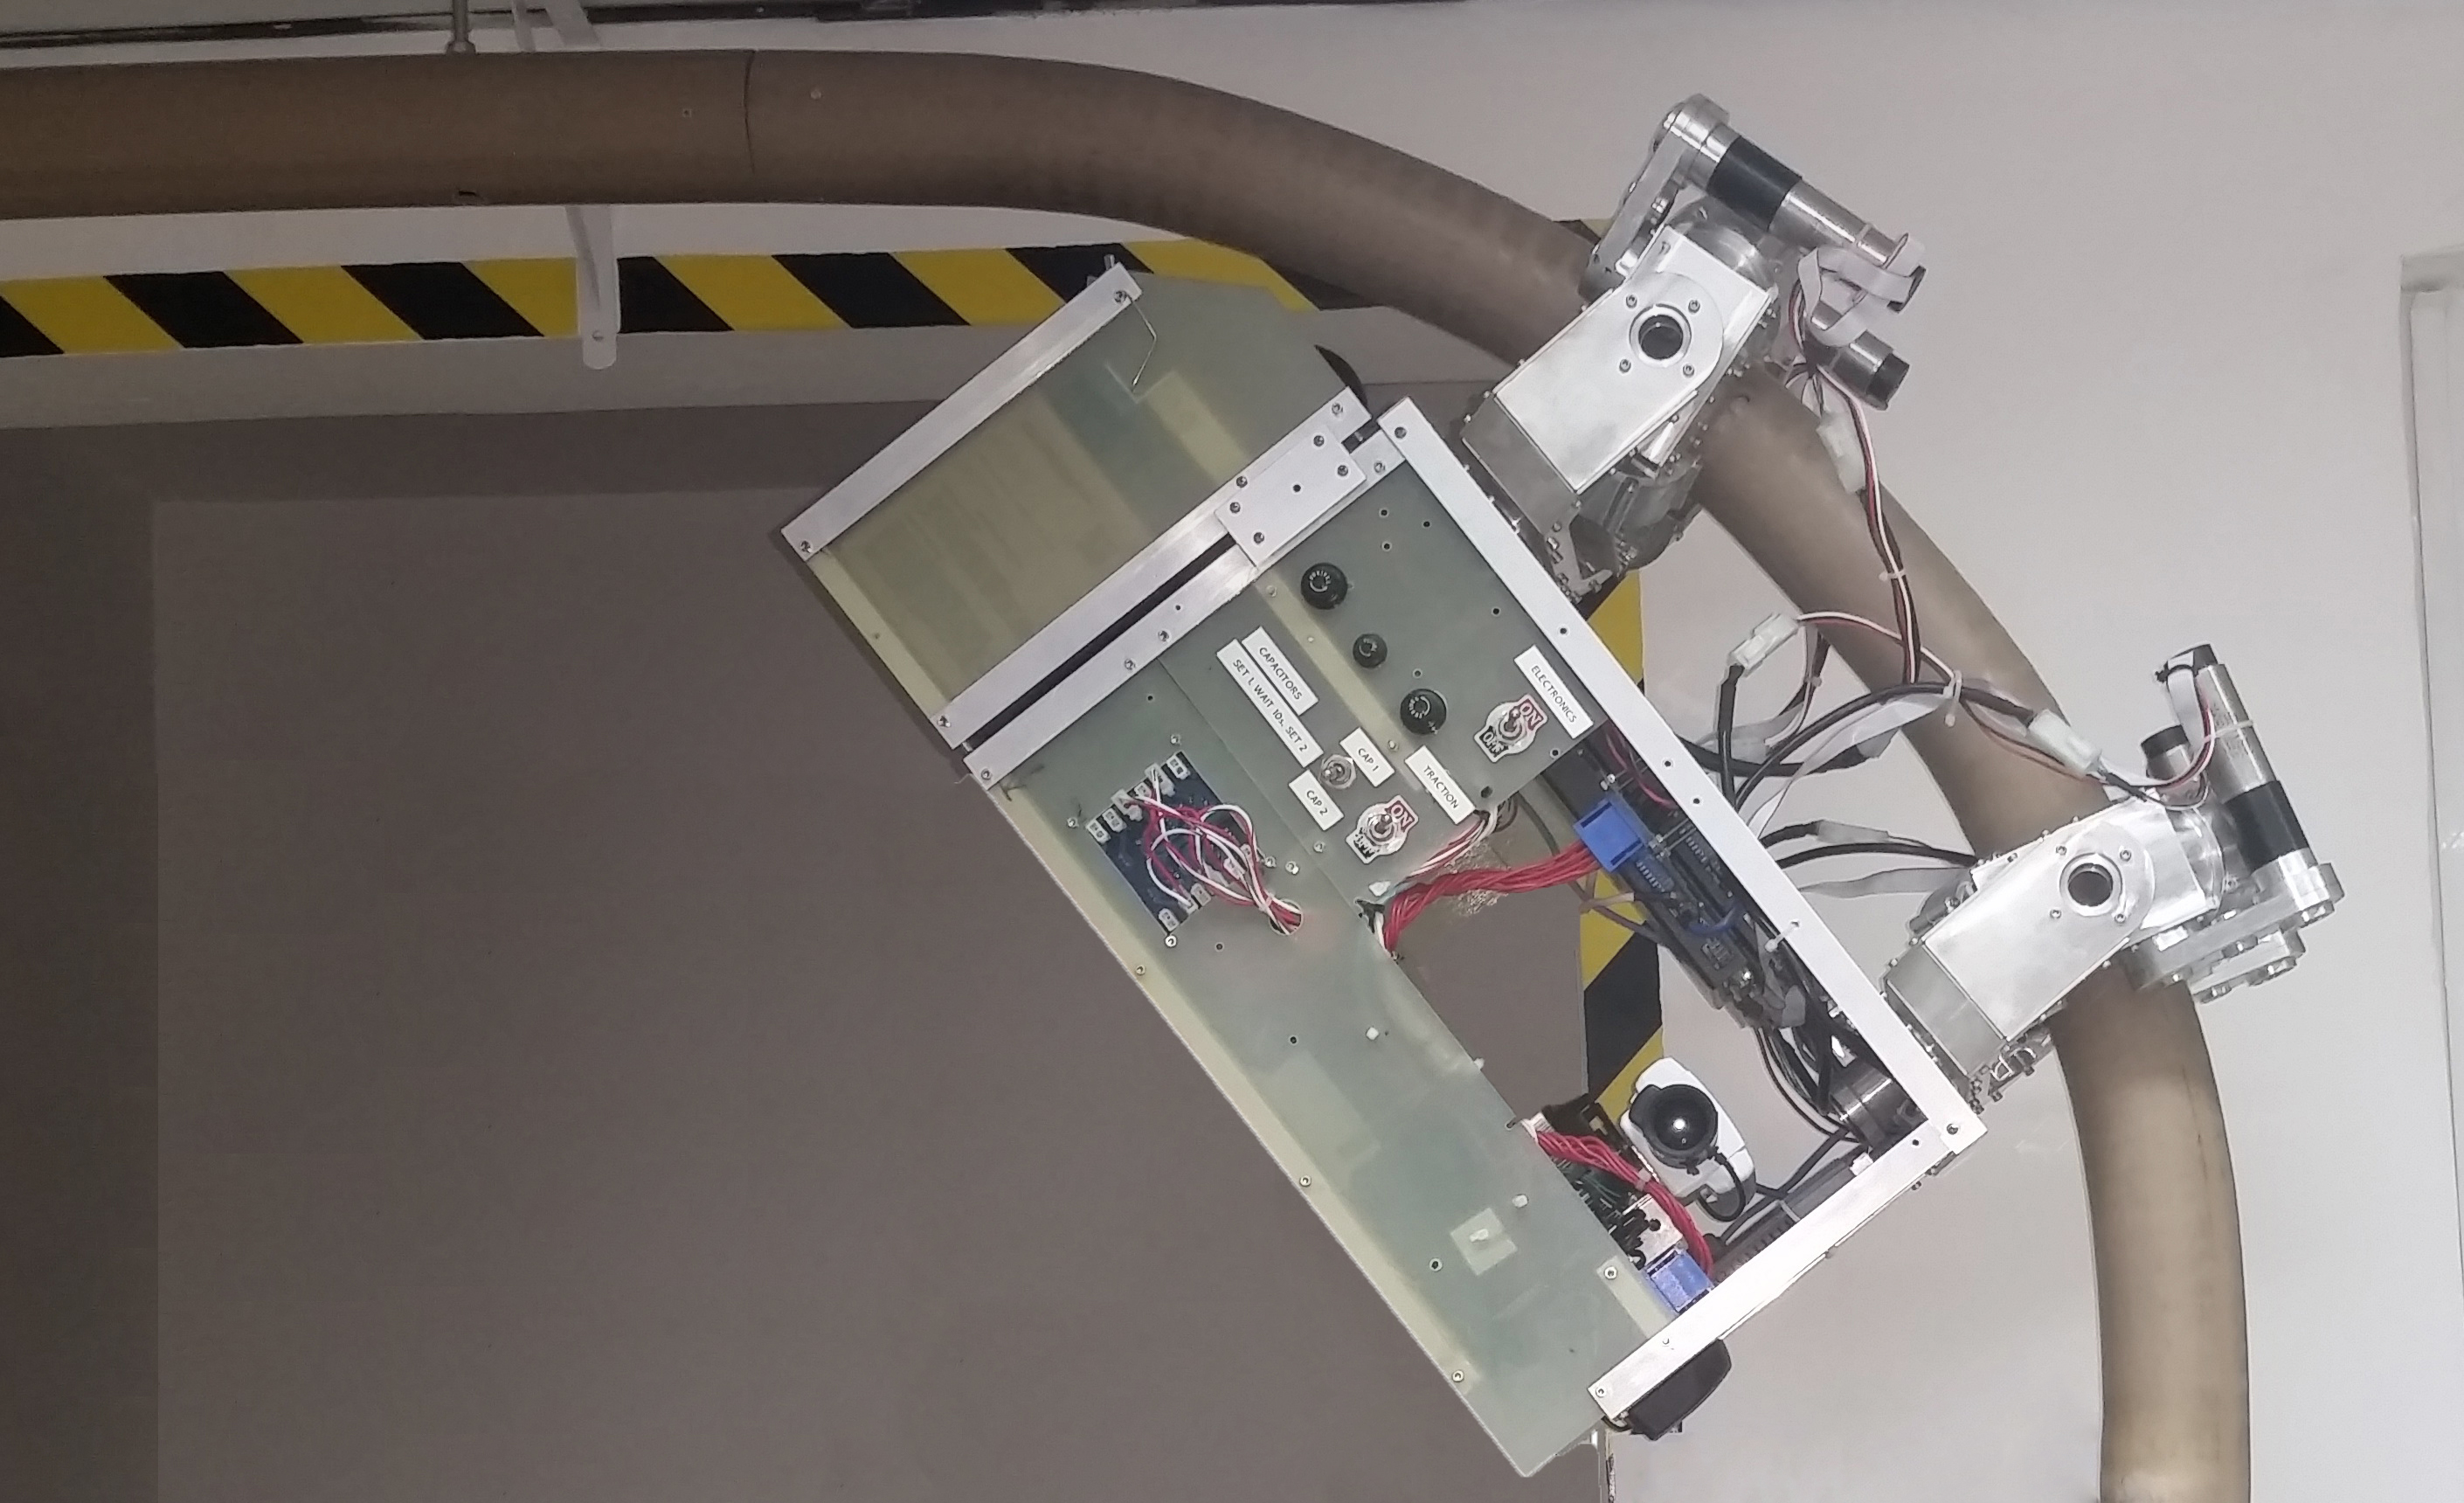
\includegraphics[width=0.5\columnwidth]{figs/SAM.jpg}
\end{center}
\textbf{Power supply:}
\begin{itemize}[<+->]
\item <1->Independent buses; 
\item <2->Battery robustness;
\item <3->Autonomy. 
\end{itemize}
}
\frame{
\frametitle{Single Autonomous Module (SAM)}
\textbf{Software architecture}
\begin{itemize}[<+->]
\item <2->Localization and 3D modelling;
\item <3->Teleoperation and User Interface.
\end{itemize}
\centering
\includegraphics[width=0.9\columnwidth]<2>{figs/DORIS3drail.png}
\includegraphics[width=0.9\columnwidth]<3>{figs/DORISui.png}
}

\section{Future work}
\frame{
\frametitle{Future work}
\begin{itemize}[<+->]
\item <1->Mission control for autonomous operation;
\item <2->VSS integration;
\item <3->Simultaneous localization and mapping;
\item <4->Hardware certification.
\end{itemize}
}
\frame{
\centering
\LARGE Thank you!
}

\end{document}
